\chapter{TINJAUAN PUSTAKA}
\label{chap:tinjauanpustaka}

% Ubah bagian-bagian berikut dengan isi dari tinjauan pustaka

\section{Penelitian Terdahulu}
\label{sec:penelitianterdahulu}

\subsection{Deep Learning}
\label{subsec:DeepLearning}

Deep learning memungkinkan model komputasi yang terdiri dari beberapa lapisan pemrosesan untuk mempelajari representasi data dengan berbagai tingkat abstraksi. Metode-metode ini telah secara dramatis meningkatkan state-of-the-art dalam pengenalan suara, pengenalan objek visual, deteksi objek dan banyak domain lainnya seperti penemuan obat dan genomik. Deep learning menemukan struktur rumit dalam kumpulan data besar dengan menggunakan algoritma backpropagation untuk menunjukkan bagaimana mesin harus mengubah parameter internalnya yang digunakan untuk menghitung representasi di setiap lapisan dari representasi di lapisan sebelumnya. Deep convolutional nets telah menghasilkan terobosan dalam pemrosesan gambar, video, ucapan, dan audio, sedangkan jaring berulang telah menyoroti data berurutan seperti teks dan ucapan.\citep{article}

% Contoh input gambar
%\begin{figure}[ht]
%  \centering

  % Ubah dengan nama file gambar dan ukuran yang akan digunakan
%  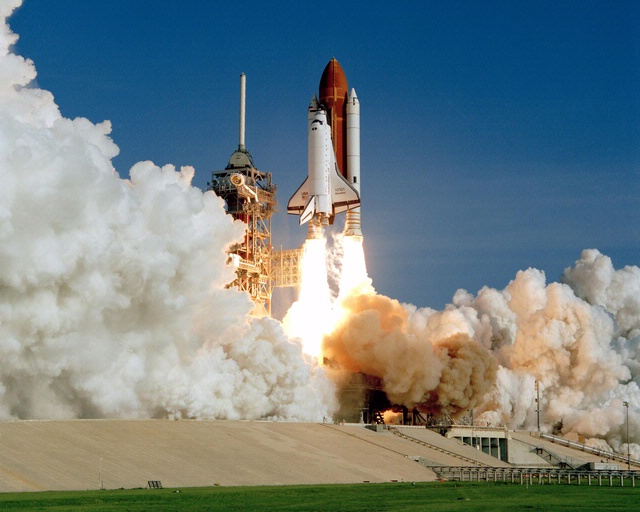
\includegraphics[scale=0.35]{gambar/roketluarangkasa.jpg}

%  % Ubah dengan keterangan gambar yang diinginkan
%  \caption{Peluncuran roket luar angkasa \emph{Discovery} \citep{roketluarangkasa}.}
%  \label{fig:roketluarangkasa}
%\end{figure}

%Roket luar angkasa merupakan \lipsum[1]

%\emph{Discovery}, Gambar \ref{fig:roketluarangkasa}, merupakan \lipsum[2]

% Per Teori Penunjang dibuat section baru

%\section{Gravitasi}
%\label{sec:gravitasi}

\subsection{YOLO}
\label{subsec:YOLO}
YOLO (You Only Look Once) merupakan sistem deteksi objek secara waktu nyata. YOLO merupakan single CNN (Convulotional Neural Network) yang secara bersamaan memprediksi lebih dari satu bounding boxes dan kelas pada satu gambar dalam satu kali pindai. Framework ini dikembangkan oleh Redmon J., Divvala S., Girshick R., Farhadi A. arsitektur jaringannya terinspirasi dari model GoogLeNet untuk klasifikasi gambar. jaringan YOLO memiliki 24 convolutional layer diikuti dengan dua layer yang terhubung.
Saat ini, ada tiga versi YOLO yaitu YOLOv1, YOLOv2, dan YOLOv3. YOLOv2 merupakan versi yang telah dikembangkan dari YOLOv1 yang mana tetap memiliki kecepatan yang sama namun dengan penambahan batch normalization, anchor boxes dan high-resolution classifier. pada YOLOv3, fitur ektraksi yang lebih baik diperkenalkan dilanjutkan dengan perkenalan 53 convolutional layer terlatih pada ImageNet. Tingkat ketelitian YOLOv3 lebih baik dari YOLOv2 namun lebih lambat karena lebih banyak layer.\citep{Redmon_2016_CVPR}

\subsection{Bangun Datar}
\label{subsec:BangunDatar}
Dalam geometri, bentuk 2D didefinisikan sebagai bangun datar yang hanya memiliki dua dimensi yaitu panjang dan lebar. Mereka tidak memiliki ketebalan apapun dan hanya dapat diukur dengan dua dimensi. Lingkaran, persegi, persegi panjang, dan segitiga adalah beberapa contoh benda dua dimensi dan bentuk-bentuk ini dapat digambar di atas kertas. Semua bentuk 2D memiliki sisi, simpul (sudut), dan sudut internal, kecuali lingkaran, yang merupakan sosok melengkung. Bentuk 2D dengan setidaknya tiga sisi lurus disebut poligon dan itu termasuk segitiga, bujur sangkar, dan segi empat.\citep{BRIBIESCA1992483}

%\subsection{Hukum Newton}
%\label{subsec:hukumnewton2}
% Contoh pembuatan persamaan
%\begin{equation}
%  \label{eq:hukumpertamanewton}
%  \sum \mathbf{F} = 0\; \Leftrightarrow\; \frac{\mathrm{d} \mathbf{v} }{\mathrm{d}t} = 0.
%\end{equation}

%\subsection{Anti Gravitasi}
%\label{subsec:antigravitasi}
\subsection{CNN}
\label{subsec:CNN}
Metode CNN (Convolutional Neural Network) merupakan pengembangan dari Metode
Multilayer Perceptron (MLP) yang didesain untuk mengolah data dua dimensi. Cara kerja CNN
memiliki kesamaan pada MLP, namun dalam CNN setiap neuron dipresentasikan dalam
bentuk tiga dimensi, tidak seperti MLP yang setiap neuron hanya berukuran satu dimensi.
Terdapat beberapa arsitektur CNN yang umum digunakan. Arsitektur tersebut yaitu
LeNet, AlexNet, ZF Net, GoogLeNet, VGGNet dan ResNet. CNN terdiri dari tiga jenis layer,
yaitu convolutional layer (Conv), pooling layer (Max pooling) dan fully-connected layer (Full
Connection). Tumpukan lapisan tersebut membentuk arsitektur dari CNN.\citep{DBLP:journals/corr/OSheaN15}
